%!Mode:: "TeX:UTF-8"
%!TEX program  = xelatex
%!BIB program = bibtex

%\documentclass[bwprint]{cumcmthesis}
\documentclass[withoutpreface,bwprint]{cumcmthesis} %去掉封面与编号页

\usepackage[framemethod=TikZ]{mdframed}
\usepackage{url}   % 网页链接
\usepackage{subcaption} % 子标题
\usepackage{float}
\usepackage{listings}
\usepackage{color}
\usepackage {mathtools}
\usepackage{algorithm}  
\usepackage{algorithmicx}  
\usepackage{algpseudocode}  
%\usepackage{amsthm}

\definecolor{dkgreen}{rgb}{0,0.6,0}
\definecolor{gray}{rgb}{0.5,0.5,0.5}
\definecolor{mauve}{rgb}{0.58,0,0.82}
\definecolor{backcolour}{rgb}{0.95,0.95,0.95}

\lstset{frame=tb,
  language=Python,
  backgroundcolor=\color{backcolour},   
  aboveskip=3mm,
  belowskip=3mm,
  showstringspaces=false,
  columns=flexible,
  basicstyle={\small\ttfamily},
  numbers=none,
  numberstyle=\tiny\color{gray},
  keywordstyle=\color{blue},
  commentstyle=\color{dkgreen},
  stringstyle=\color{mauve},
  breaklines=true,
  breakatwhitespace=true,
  tabsize=3
}

%参考文献引用命令
%\newcommand{\upcite}[1]{\textsuperscript{\textsuperscript{\cite{#1%}}}}
\renewcommand{\algorithmicrequire}{\textbf{Input:}}  % Use Input in the format of Algorithm  
\renewcommand{\algorithmicensure}{\textbf{Output:}} % Use Output in the format of Algorithm  

\title{基于指纹特征点方向梯度编码和匈牙利算法的指纹匹配分类模型}
\tihao{题号}
\baominghao{报名号}
\schoolname{武汉理工大学}
\membera{许鸢飞}
\memberb{李想}
\memberc{尹可汗}
\supervisor{指导老师}
\yearinput{2020}
\monthinput{07}
\dayinput{24}


%\graphicspath{{./figures/}} %图片在当前目录下的figures还有目录

\begin{document}

\maketitle
\begin{abstract}
	本文根据指纹学基本知识和机理建立了基于指纹核心点和细节特征点信息的编码,建立了二分图模式的匹配分类模型,利用图像特征点信息和图像方向场梯度,通过匈牙利算法给出了上述问题结果。
   
   针对问题一,该问题需要设计一种能反映指纹基本特征的编码方式。我们首先进行原始图像的预处理,\textbf{通过归一化、分割、Gabor滤波增强、二值化等方法},将原始图像转换为便于提取特征信息的清晰图像。考虑到\textbf{指纹采集过程发生的旋转现象},我们建立了\textbf{图像旋转校正模型},通过OpenCV自带函数cvFitellipse2和cvBoxPoints找到图像的最小外椭圆和外接矩形,将图像转换成竖直方向的状态,接着我们应用\textbf{Poincare Index索引法}找出指纹的中心点,并基于中心点建立二维坐标系。编码方式建立在中心点与细节点的关系上,\textbf{分别以细节点到中心点的横轴相对距离与纵轴相对距离,细节点的类型和经过细节点的指纹脊线斜率作为四个维度设计编码},编码的顺序取决于中心点到细节点的几何距离,\textbf{每张图片共选取20个特征点,所有编码均控制为140个字节大小。}
   
   针对问题二,该问题需要比较不同指纹之间的\textbf{相似程度}。根据指纹学知识,指纹的特征取决于\textbf{细节点与中心点的相对位置,类型以及其所在脊线切线的方向}。在第一问编码的基础上,通过\textbf{特征点和与其最近邻的一个特征点}构建匹配收益矩阵。使用\textbf{匈牙利算法}求解二部图之间的最大匹配情况,然后利用匹配结果计算总收益,归一化后指纹图像间的匹配度。1代表完全匹配,0代表完全不匹配。\textbf{在前六张图像中,其中2和6匹配度较高为0.454979,而图像2和图像1的匹配度较低为0.112406,其余匹配度在附录中给出,结果符合原始信息}。对该模型进行\textbf{灵敏度分析},发现将节点数由20变为15或10的情况下,结果的平均误差和最大误差变化不大,\textbf{说明该结果具有稳定性}。
   
   针对问题三,根据指纹学知识,\textbf{中心点和三角点}对于指纹的分类而言是一个重要依据,同时\textbf{指纹中心附近的方向场和梯度能准确的反映我们指纹曲线的趋势和方向},能便于我们更好的进行分类,从以上两个方面,我们利用\textbf{Sobel算子和高斯滤波}的获取了指纹图像方向场梯度,而\textbf{指纹中心点和三角点则就是方向场梯度骤变的交叉点},然后在用\textbf{poincare验证和提取}出对应坐标,借助前面的编码模型基础和匹配算法从而对16个指纹图像进行了准确分类,\textbf{最后结果为两个中心点的当中7,8为螺旋型,14号为斗型,其余单中心点的图像中1,4,9,15为弓型,2,3,5,6,10,11,12,13,16为箕型,并求出了指纹的旋转方向梯度。}
   
   本文的优点在于:1.将指纹的特征点和相似度匹配分类转换为了二分图之间的最大匹配模型的问题。2.在指纹分类和匹配上既考虑了特征点的信息还考虑了图像的方向梯度问题。
   \keywords{
	   poincare索引\quad
	   二分图匹配  \quad
	   匈牙利算法\quad  
	   方向场梯度\quad  
   }
   \end{abstract}


%目录
\tableofcontents
\newpage

\section{问题重述}
\subsection{问题背景}
指纹是指人的手指第一节手掌面皮肤上的乳突线花纹,由于指纹具有唯一性、稳定性和可采集性等特点,指纹也被称为人体身份证。指纹识别技术是目前最为可靠的身份认证方法之一,被广泛用于边境检查,贵重物品保管,重要部门安保,网络安全防护等领域中,指纹是应用最普遍,识别率最高,最容易被接受的个人身份认定方法。

目前大部分指纹自动识别方法都是基于细节特征的,即提取细节点作为特征来表征指纹图像,通过这些特征进行识别,指纹的特征可分为三类:全局特征,局部特征和细微特征,且对任一指纹的识别要满足至少两类特征,这种方法具有信息储存量小,识别速度快等优点。

\subsection{待解决的问题}
1.给出一种不超过200字节的,用来描述相应指纹的基本特征的指纹密码

2.给出每一幅指纹图像的指纹密码,基于指纹密码的表示给出一种能够比较不同指纹间异同和相似度的方法。

3.对附件中16个指纹进行对比和归类,并给出相应的依据和结果。

\section{模型假设}
\begin{enumerate}
	\item 指纹相对完整,指纹区域内至少包含一个中心点。
	\item 假设所给图像是噪声较小,对于图像特征点的提取编码不会出现较大的影响。
	\item 尽管由于按压深浅或其他原因导致的图像清晰程度有所不同,但经过图像增强或者修复后,靠近中心点的核心区域细节点缺失较少。
\end{enumerate}

\newpage
\section{符号说明}

\begin{center}
	\begin{tabular}{ccccc}
		\toprule[1.5pt]
		符号 & 含义\\
		\midrule[1pt]
		$I$$(i,j)$ & 像素点$(i,j)$的灰度值\\
		$M_{i}$,$V_{i}$ & 像素点灰度值的平均值及方差\\
           $E$$(i,j)$ & 滤波后图像的灰度值\\
           $T$        &  二值化方法的阈值\\
           $\theta(k) $        & 封闭曲线上第$k$个点的方向,$k$取1,2,...\\
           $\partial$$x(i,j)$,$\partial$$y(i,j)$ &像素点在$X$,$Y$方向的梯度\\
           $W_{\phi}$  & 滤波器的尺寸\\
		\bottomrule[1.5pt]
		注:表中未说明的符号以首次出现处为准
	\end{tabular}
\end{center}


\section{问题一模型的建立与求解}
\subsection{问题分析}
%插入参考文献\upcite{bib:one}。
该问题要根据一般问题,给出指纹识别方法的一般性步骤。针对该问题,首先要对指纹学的基本概念进行了解,例如指纹的3大类型和9种形态,这种分类方法也被称为二级分类法。

由于指纹的唯一性特性,在设计指纹密码时应以指纹的特异性特征为依据,指纹的特异性特征包括指纹的种类,特征点的数量及类型,脊线的走势及长度等等。为了对指纹的特征点进行编码处理,我们需把提取出的特征向量放在一个字符串中,并根据特征向量的数量和类型给出编码格式,并作出数学解释。

需要注意的是,由于题目提供的指纹图像的大小,深浅,方向不一致,我们首先需要对各个图像进行一致化处理,由于现实中指纹采集的角度和方向不可能完全一致,我们提出的编码方式必须不受图像旋转的影响。

\subsection{前期准备}

\subsubsection{相关概念解释}
指纹学是研究掌面肤纹生理特征、纹理结构及其收集、显现、储存、分类与识别的原理和方法的科学.在介绍我们的方法之前需要对指纹学相关概念作出解释。

\textbf{指纹的基本特征}
指纹是指收支正面皮肤凹凸不平的纹路,纹路中隆起的部分是手指真皮向表皮乳突形成的褶皱,又被称为\textbf{指纹脊线(ridge)},指纹脊线之间的凹陷部分被称为\textbf{指纹谷线(furrow)},不同指纹间纹线的数目和走势是存在差异的,且纹线数目,走势不会随年纪的增长而发生显著变化\cite{赵应丁2006基于灰度指纹图像的指纹特征提取算法研究}。
\begin{figure}[!h]
	\centering
	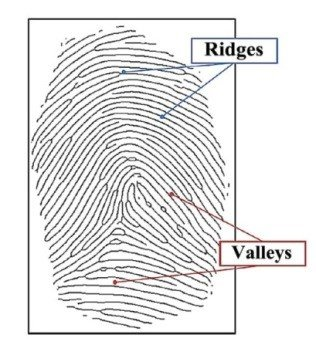
\includegraphics[width=0.6\textwidth]{RidgesValleys.png}
	\caption{脊线和谷线}
	
\end{figure}

\textbf{指纹的全局特征}
指纹的全局特征包括人眼直接可以观察到的特征,比如指纹纹型,模式区,中心区,三角区及纹线数目等。
最基本的分类方法是按照纹路纹型的分类法,目前比较常见的方法是依据指纹的中心模式区和三角模式区划分的,一般依据指纹形状的不同将指纹分为3大类(\textbf{弓形纹(Arch)},\textbf{箕型纹(Loop)}和\textbf{螺旋型纹(Whorl)}),9种形态(弧形,帐形,左簸箕形,游簸箕形,环形,螺形,囊形,双簸箕形,杂形)。
\begin{figure}[!h]
	\centering
	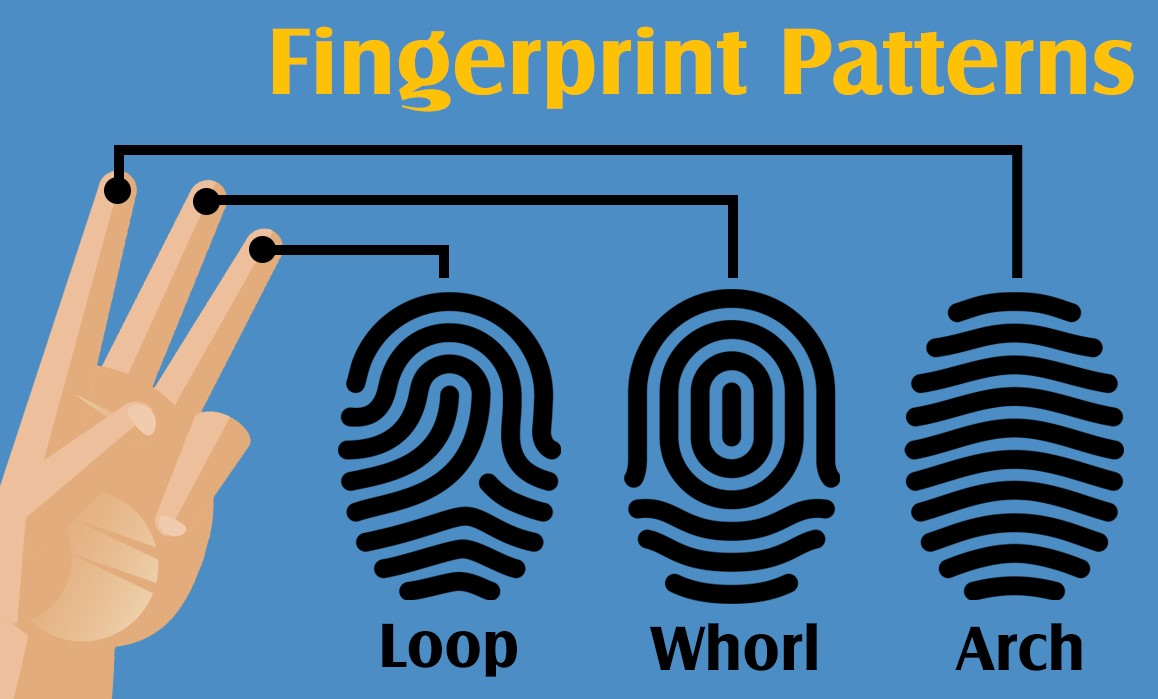
\includegraphics[width=0.8\textwidth]{fingerprintType.jpg}
	\caption{纹型示意图}
	
\end{figure}

\textbf{指纹的局部特征}
脊线上有一些能够是指纹图像获得更高区分度和可信度的点,这些点夹杂在脊线与谷线之间,被称作细节点。
我们在下图给出了常见的细节点类型,并作出解释。\par
\textbf{端点(ridge ending)}:一条脊线的终结点.\par
\textbf{分叉点(bifurcation)}:一条指纹纹线在此点分成两条或者更多条的指纹纹路.\par
湖(lake):存在两条或者两条以上的连接两个分叉点的纹线.\par
独立脊线(independent ridge):一条较短但不足以成为一点的纹线.\par
孤岛(dot):一条较短的纹线,可以看做是一点.\par
毛刺(hook):一条指纹文献在此处分出一条较短但不至于成为脊线的纹线.\par
交叉点(ridge crossing):四条纹线汇聚在此点.\par
需要注意的是,人的指纹中还有很多特殊的细节特征,但是大部分特征是难以提取或者不能作为匹配特征的,在上述细节点中,端点和分叉点的概率是所有局部特征的80$\%$以上,所以本文主要关注这两种局部特征.
\par

当采用高分辨率传感器的时候,我们可以提取脊线上更细微的特征,但这样的手段一般适用于及其重要或者安全等级最高的防护设施中,因此,本文对细微特征不做考虑。
\begin{figure}[!h]
	\centering
	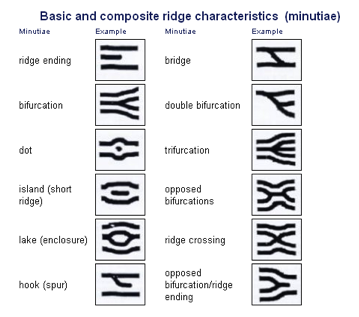
\includegraphics[width=0.8\textwidth]{class.png}
	\caption{细节点类型示意图}
	
\end{figure}

\subsubsection{图像预处理}
在图像的形成和运输过程中,由于受到诸如系统噪声,曝光不足等的影响,获取到的图像可能与原始图像之间存在差异,为了更好的提取指纹图像中的信息,我们需要对原始图像进行预处理。
指纹图像处理的主要流程如图\ref{fig:preprocess}:
\begin{figure}[!h]
	\centering
	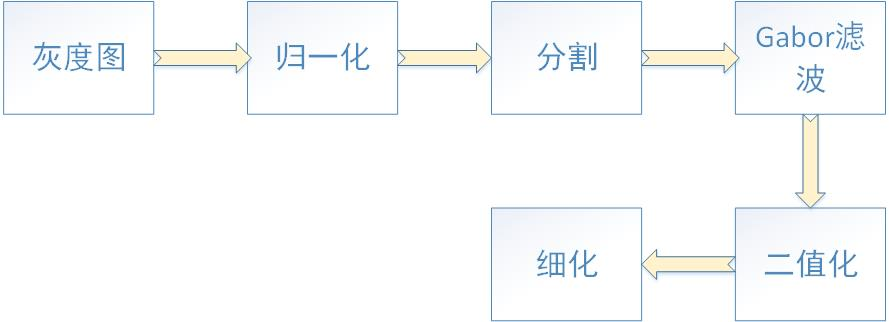
\includegraphics[width=0.8\textwidth]{preprocess.jpg}
	\caption{预处理流程图}
	\label{fig:preprocess}
\end{figure}

\textbf{归一化和切割}

由于指纹按压形成的过程中的手指压力和强度不同,不同图像区域之间的清晰度会有明显差异,归一化调整的是指纹灰度均值和其方差,调整到标准状态并屏蔽不必要的噪声。\par
1.我们将指纹分成W*H个小块,W,H分别表示将指纹图像的宽度和长度切成的份数。设图像中的像素点的弧度制为$I(i,j)$,归一化后的图像灰度值用$G(i,j)$来表示,灰度平均值和方差分别用$M_{i}$和$V_{i}$来表示,则归一化的算法如下:
\begin{equation}
M_{i}=\frac1{WH}\sum_{i=0}^{H-1}\sum_{j=0}^{W-1}I(i,j)
\end{equation}
\begin{equation}
V_{i}=\frac1{WH}\sum_{i=0}^{H-1}\sum_{j=0}^{W-1}({I(i,j)-M_{i})^2}
\end{equation}

2.指订期望的图像方差和平均值后,算出归一化后的图像灰度值$G(i,j)$\par

\begin{equation}
G(i,j)=
\begin{cases}
M_{0}+\sqrt{\frac{V_{0}\left(I(i, j)-M_{i}\right)^{2}}{V_{i}}},& I(i,j)>M_{i}\\
M_{0}-\sqrt{\frac{V_{0}\left(I(i, j)-M_{i}\right)^{2}}{V_{i}}},& I(i,j)<M_{i}\\
\end{cases}
\end{equation}


其中,$M_{0}$,$V_{0}$为期望的平均值和方差。\par

\textbf{分割}

分割图像基于块特征的指纹图像分割,本文采用均值方差法,该算法基于背景区灰度方差小,而指纹区方差大的思想,将指纹图像分成块,计算每一块的方差,如果该房差小于阈值则为背景,否则为前景.具体步骤分为以下三步:\par
1.将图像分为$N×N$的方块。

2.计算出每一块的均值和方差。

3.将该块方差与阈值进行比较。

\textbf{Gabor滤波增强}

Gabor滤波器作为带通滤波器,因其空域内具有良好的方向选择性及频域内良好的频率选择性而在计算机视觉领域尤其是问你分析方面得到了广泛的应用\cite{贺颖2010应用}。在指纹图像中,对于灰度指纹图像,脊线和谷线在局部的小领域中可被认为是正选波形状,具有一定的频率和方向。\par
利用Gaborl滤波器良好的对方向和频率的选择性滤波是图像增强的一个很好地方案,实验表明,以Gabor函数的偶分量实部为模板,脊线与谷线形成的近似正弦波的频率为频波器的频率,以指纹的局部方向构建的滤波器,去噪效果非常好,滤波后的指纹图像的灰度直方图呈现明显的双峰形势。\par
Gabor滤波器的形式如下:
\begin{equation}
h(x, y: \theta, f)=\exp {\frac{-1}{2}[\frac{{x^\prime}^{2}}{\delta_{x}^{2}}+\frac{{y^\prime}^{2}}{\delta_{y}^{2}]} \cos (2\pi fx)}
\end{equation}

其中:$$x^\prime=x\sin{\theta}+y\cos{\theta}$$
$$y^\prime=x\cos{\theta}-y\sin{\theta}$$
滤波后图像的灰度值为
\begin{equation}
E(i,j)=\sum_{x=\frac{W}{2}}^{\frac{W}{2}}\sum_{y=\frac{W}{2}}^{\frac{W}{2}}h(x,y:\varphi(i,j),f(i,j))g(i-x,j-y)
\end{equation}

Gabor 滤波增强后的效果前后对比如图\ref{fig:enhance}所示:

\begin{figure}[H]
	\begin{minipage}[t]{0.45\textwidth}
		\centering
		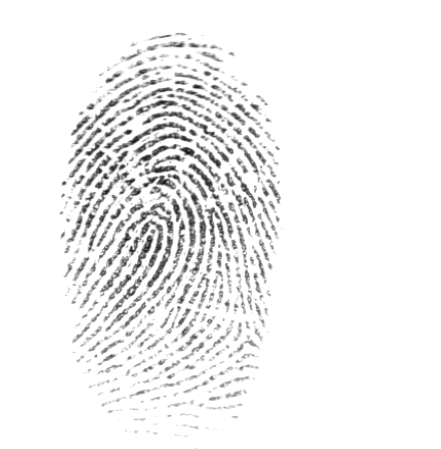
\includegraphics[width=0.99\textwidth]{original.png}	
		\label{fig:original}
           \caption{滤波增强前}
	\end{minipage}
	\qquad
	\begin{minipage}[t]{0.45\textwidth}
		\centering
		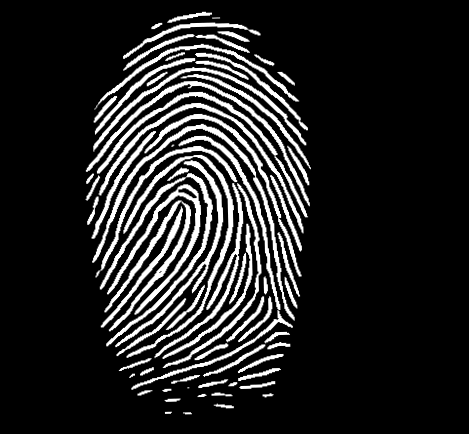
\includegraphics[width=0.99\textwidth]{enhanced.png}
		\label{fig:enhanced}
          \caption{滤波增强后}	
	\end{minipage}
	\label{fig:enhance}
	\caption{滤波增强前后对比}	
\end{figure}


\textbf{图像二值化处理}

指纹图像二值化处理作为指纹预处理过程的一部分,是进行指纹图像细化处理的基础,二值化后的图像其几何性质只与0和1的位置有关,不在设计像素的灰度值,使得处理变得简单,这给存储和处理带来了方便。二值化处理后的图像有几个基本要求:
\begin{enumerate}
	\item  脊线中不出现空白
	\item 二值化后的脊线基本保持原来的指纹的特征
	\item 指纹的纹线不应有太多的间断和相连
	\item 指纹纹线间的间距应大致相同
\end{enumerate}
我们使用自适应阈值二值化的思想,对每块指纹图像,选取的阈值应尽量使该块图像内大于该阈值的像素点数小于该阈值的像素点数。
一般灰度图像二值化的变换函数用下列公式表示:
\begin{equation}
f(x)=
\begin{cases}
1& \text{x>=T}\\
0& \text{x<T}
\end{cases}
\end{equation}
$T$为阈值\par
自适应阈值算法是利用固定阈值算法的思想,根据图像的每一部分的敏感度来调整阈值。本文首先把图像分为若干个方块,每一块根据自己的阈值进行二值化,这种算法充分利用了指纹图中脊线和谷线宽度大致相同的特点,即二值化后黑白像素的个数也大致相同,首先利用固定阈值算法的特点对指纹图像中的每块确定一个大致的阈值,然后再利用自适应的思想对阈值进行准确地调整,即阈值的取值合适时图像时最光滑的,0-1之间的转换次数最少。
$$ T=\frac{1}{w_{2}}\sum_{u=i-\frac{2}{w}}^{i+\frac{2}{w}}\sum_{v=j-\frac{2}{w}}^{i-\frac{2}{w}}\times G(i,j)$$

\subsection{图像旋转校正特征点编码模型}
\subsubsection{图像旋转校正}
实际上,在采集指纹图像时,手指与采集仪器之间往往并不是平行接触的,这就导致得到的指纹图像发生旋转倾斜的情况,图像的大小比例也会发生失调,并且无法找到图像的对称轴。
yin和ye等提出了一种图像旋转矫正的方法\cite{尹婉琳2014指纹图像的旋转校正与分类},利用OpenCV自带函数$cvFitellipse2$和$cvBoxPoints$找到最小的外椭圆和矩形。当矩形存在一定的倾斜角度时,无需判断椭圆即可确定指纹发生了偏转;当矩形未偏转时,若椭圆是倾斜的,且其长径远远大于短径,则说明指纹需要进行旋转校正。
指纹分类算法流程图为:
\begin{figure}[!h]
	\centering
	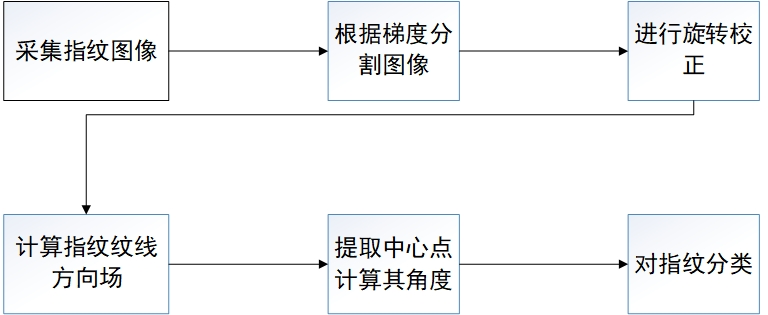
\includegraphics[width=0.8\textwidth]{rotateProcess.jpg}
	\caption{旋转流程图}
\end{figure}

首先我们将指纹图像的最大外接正矩形按照左下,右下,左上,右上四个方向分为1,2,3,4标注的4个区域,若发生了偏转,则必然会存在某两个对称区域存在相对较多的背景点。我们可以利用这一特点验证椭圆校正方法是否判断正确。另外,若在实际应用中遇到指纹图像几乎充满了整个所在矩形,而只有一个方向存在很多背景点,则无论椭圆是否有偏转都不需要校正图像。\par

得到了指纹的偏转角度后,调用OpenCV库中的$cvWAaRPAffine$函数对整个指纹区域进行仿射变换,进而完成指纹图像的旋转校正,再次基础上计算指纹的方向场,角度范围在[0~π]之间,算法流程图如图\ref{fig:adjustProcess}:
\begin{figure}[!h]
	\centering
	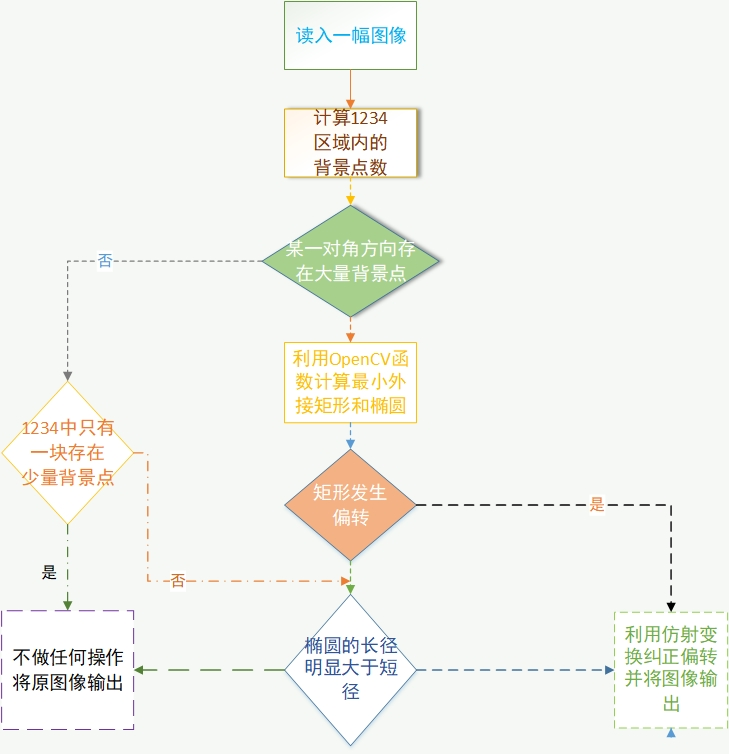
\includegraphics[width=0.8\textwidth]{adjustProcess.jpg}
	\caption{校正偏角算法流程图}
	\label{fig:adjustProcess}
\end{figure}

\subsubsection{中心点的提取}
在指纹图像中,奇异点是一种不同于细节点的宏观特征,其数目和相对文职可以帮助判断指纹的类别,根据奇异点领域内的脊线分布情况,可分为中心点和三角点\cite{张祖泷2012指纹奇异点精确定位新方法}。

奇异点提取是指纹图像处理中的一个重要部分,它可以作为指纹分类和识别过程中的定位基准点,根据其分布特性可以对指纹图像做粗分类,故提取的准确性直接影响到指纹分类和细节匹配的准确率.

本文采用主流的Poincare索引法,该方法不会受到图像旋转的影响,即检测过程补语像素点在图像中的绝对位置和方向相关.Poincare所以发是根据Poincare索引值对像素点的性质进行区分,如图\ref{fig:poincare}所示,$C$是方向图$D$中围绕像素点$(x,y)$的一条封闭曲线,$V_{1}$到$V_{9}$表示曲线C上的像素点的方向矢量.
\begin{figure}[!h]
	\centering
	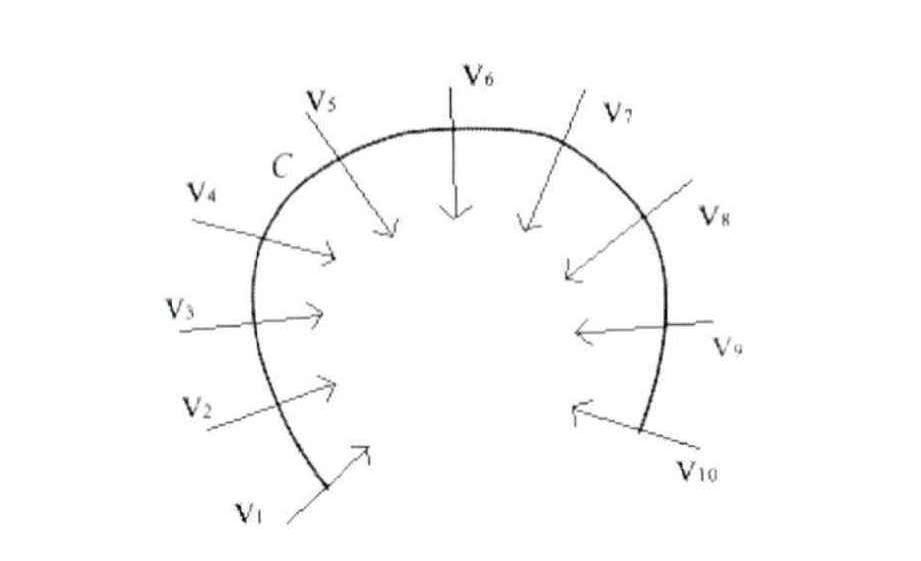
\includegraphics[width=0.8\textwidth]{poincare.jpg}
	\caption{Poincare索引法原理图}
	\label{fig:poincare}
\end{figure}
$Poincare$索引值的计算公式为:
$$Poincare(x,y)=\frac{1}{2\pi}\sum_{k=0}^{N}\Delta(k)$$
其中:
\begin{equation}
\Delta(k)=
\begin{cases}
\delta(k), & |\delta(k)|\le \frac{\pi}{2} \\
\delta(k)+\pi, & \delta(k)\leq \frac{-\pi}{2} \\
\delta(k)-\pi,  & otherwise   
\end{cases}
\end{equation}
$$\delta(k)= \theta(k^\prime)-\theta(k) $$
$$k^\prime = (k+1)modN $$
式中,$\theta(k)$的意义为编号为$k$的点的方向值,$N$的意义为组成曲线$C$的点的数量

本文选取了3×3的邻域模板用于检测所有奇异点。
我们发现采用Poincare索引法求得的所有奇异点中,存在大量靠近图像边缘的伪奇异点,为此我们给每张图像划取了一个大致范围,并去掉范围外的奇异点,这种方法的可取性在于:在获取指纹图像时,由于按压深浅或者采集传导过程中的随机因素,图像边缘会出现大量端点,去除这些奇异点有助于使处理后的图像更加可靠。

\subsubsection{编码方法}
本题中我们得到的图像为分辨率640×480的大小为300$kb$的图像,我们默认以后获得的图像也是同样大小及分辨率的图像或者可以被转化为这种样式的图像。
在对整个16幅图像进行了图像旋转校正之后,我们得到了近似于正向,即在指纹录取时得到的最规范的图像。  
在前期的工作中我们已经得到各原始指纹图像二值化后的新图像,同时我们找到了各图像的中心点以及细节点。
由此我们提出了一种指纹密码的编码方式:\par
第一步:以中心点为原点(用$O_{i}$表示,$i$=1,2,...16),借助与旋转后图像边缘平行的直线,建立二维平面直角坐标系。\par
第二步:在所有细节点中,选取离中心点最近的20个细节点,并画出这些点的大致范围。\par
第三步:求出所有细节点与中心点在横坐标轴和纵坐标轴上的相对距离,距离为正表示该细节点在中心点的指向正半轴的方向上,距离为负表示该细节点在中心点的指向负半轴的方向上,由此我们获得了各细节点相对于中心点的距离,也就是它们的相对坐标,分别用$\delta$$x$和$\delta$$y$ 表示\par
第四步:将细节点分类,端点记为0,分叉点记为1.\par
第五步:依据建立的二维直角坐标系,计算细节点沿脊向方向的切线的斜率,由于图像已被二值化,我们通过以下方法近似处理:对于端点,我们选择同一条脊线上距离该端点最近的两个像素点,以此三点确定一条直线的斜率,通过最小二乘法进行拟合;对于分叉点,我们选择的是两条分叉路径之中偏离中心点的一条直线,求解斜率方法与端点相同。\par
最小二乘法确定了线性回归方程为:$$\hat{y}=a+bx$$
其中:
\begin{equation}
\hat{b}=\frac{\sum_{j=1}^{n} x_{j} y_{j}-n \bar{x} \bar{y}}{\sum_{j=1}^{n} x_{j}^{2}-n \bar{x}^{2}} \quad
\hat{a}=\bar{y}-\hat{b} \bar{x}
\end{equation}
推到过程不在此赘述。
我们的编码设计有4个维度,分别是与中心点在横坐标上的相对距离$x$,与中心点在纵坐标上的相对距离$y$,细节点的类型$t$及经过细节点的脊线切线的斜率。
需要说明的是编码的顺序按照距离中心点距离,由小至大的顺序排列,该距离为二维空间几何距离。
此方法表示的特征点信息的编码格式: 
\par 

%\begin{tabular}{|c|c|c|c|c|c|c|c|c|c|r|}
%	\hline
%	$\delta$$x_{1}$ & $\delta$$ y_{1}$ & $t_{1}$ & $k_{1}$ & $\delta$$ x_{2}$ & $\delta $$y_{2}$ & $t_{2}$ & $k_{2}$ & ... & $t_{20}$ & $k_{20}$\\
%	\hline
%\end{tabular}

\begin{equation}       %开始数学环境
Code= \left(                 %左括号
\begin{array}{ccccccccccr}   %该矩阵一共3列,每一列都居中放置
	\delta x_{1} & \delta y_{1} & t_{1} & k_{1}, & \delta x_{2} & \delta y_{2} & t_{2} & k_{2}, & ... & t_{20} & k_{20}
\end{array}
\right)                 %右括号
\end{equation}

其中$\delta x_{1}$表示存放细节点与中心点在横轴上的相对距离,占用2个字节,其中$\delta y_{1}$表示存放细节点与中心点在纵轴上的相对距离,占用2个字节,$t_{1}$表示存放细节点的类型,占用一个字节,$k_{1}$表示经过细节点的脊线切线斜率,占用2个字节。任意图像的指纹密码共保存20个特征点,占用$20×(1+2+2+2)=140$个字节。


\subsection{模型求解}
\subsubsection{图像腐蚀前后背景分离}
录取的指纹在边缘部分常常是模糊不清的,图像同时伴随大量噪声,我们首先对原指纹图像进行了腐蚀与膨胀,其目的在于消除噪声,寻找图像中明显的极大值或极小值区域。
\begin{figure}[H]
	\begin{minipage}[t]{0.5\textwidth}
		\centering
		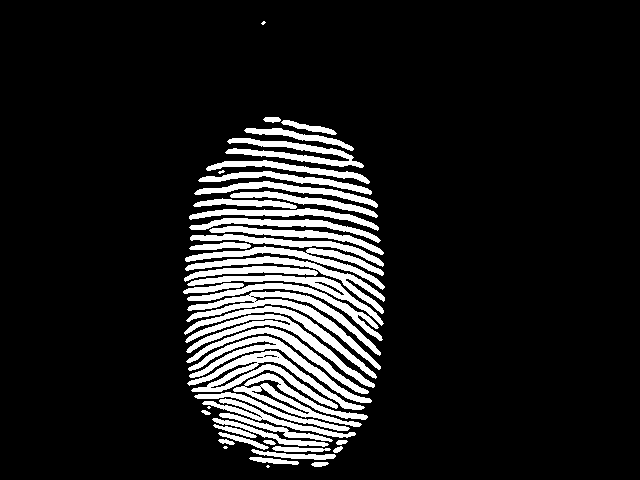
\includegraphics[width=0.99\textwidth]{01mask.png}
		\label{fig:01mask}
		\subcaption{图像膨胀前}
	\end{minipage}
	\qquad
	\begin{minipage}[t]{0.5\textwidth}
		\centering
		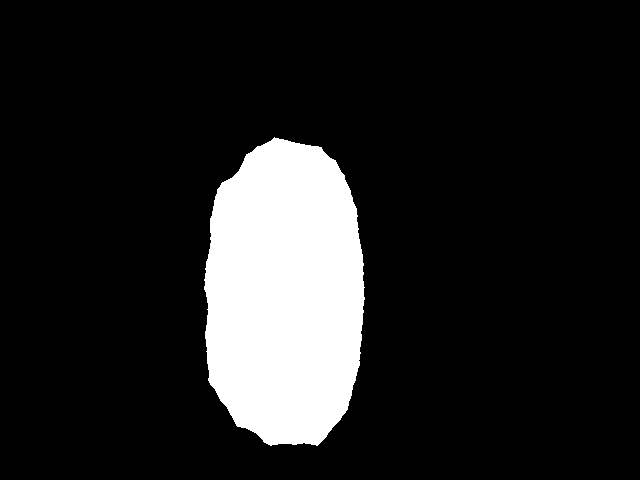
\includegraphics[width=0.99\textwidth]{01edge_filter.png}
		\label{01edge_filter}
		\subcaption{图像膨胀后}
	\end{minipage}
	\label{}
	\caption{图像膨胀前后对比}
\end{figure}

\subsubsection{图像二值化与特征点提取}
接下来我们对图像进行进一步处理,划分了图像包含了大量细节点的核心区域。我们使用Poincare index索引法求出了图像的中心点(以黄色点表示),并利用二值化后图像的性质,找到了指纹的端点和分叉点(分别以蓝色点和红色点表示),下图给出了图片一经过处理后核心区域的图像:
\begin{figure}[!h]
	\centering
	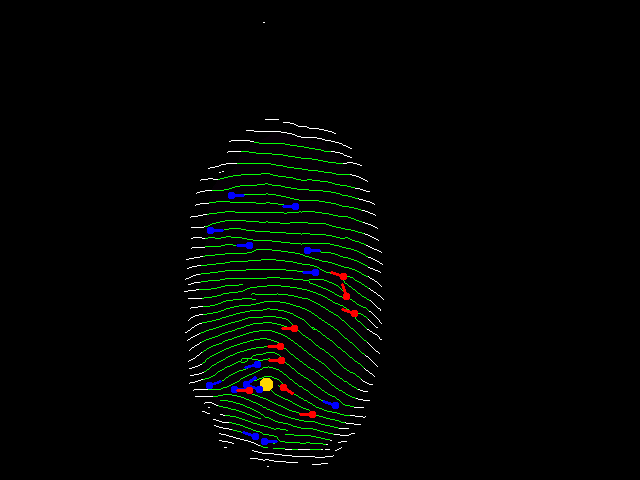
\includegraphics[width=0.8\textwidth]{01result}	
	\caption{图片一核心区域示意图}
\end{figure}

接下来利用中心点定位编码方法,我们计算出图像一中各细节点到中心点在横轴与纵轴上的相对位置,和通过细节点的与脊线相切的直线的斜率,细节点的编号按照到中心点的距离从小到大进行排列.

中心点与细节点之间的距离采用欧几里得距离公式
\begin{equation}
D_{i}=\sqrt{(\delta x)^2+(\delta y)^2}.
\end{equation}

表\ref{tab:feature}列出了图一中距离中心点最近的20个细节点的特征

% Table generated by Excel2LaTeX from sheet 'Sheet1'
\begin{table}[htbp]
	\centering
	\caption{第一个图像的特征点相对位置、角度和类别}
	  \begin{tabular}{crrrr}
	  \toprule
			& \multicolumn{1}{c}{\textbf{row}} & \multicolumn{1}{c}{\textbf{col}} & \multicolumn{1}{c}{\textbf{angle}} & \multicolumn{1}{c}{\textbf{class}} \\
	  \midrule
	  \textbf{0} & 389   & 259   & -2.81984 & 0 \\
	  \textbf{1} & 387   & 283   & 0.588003 & 1 \\
	  \textbf{2} & 390   & 249   & 3.141593 & 1 \\
	  \textbf{3} & 384   & 246   & -0.588 & 0 \\
	  \textbf{4} & 364   & 257   & 2.819842 & 0 \\
	  \textbf{5} & 360   & 281   & 3.141593 & 1 \\
	  \textbf{6} & 389   & 234   & 0     & 0 \\
	  \textbf{7} & 346   & 280   & 3.141593 & 1 \\
	  \textbf{8} & 436   & 255   & -2.81984 & 0 \\
	  \textbf{9} & 414   & 312   & 3.141593 & 1 \\
	  \textbf{10} & 385   & 209   & -0.32175 & 0 \\
	  \textbf{11} & 441   & 264   & 0     & 0 \\
	  \textbf{12} & 328   & 294   & 3.141593 & 1 \\
	  \textbf{13} & 405   & 335   & -2.81984 & 0 \\
	  \textbf{14} & 313   & 354   & -2.81984 & 1 \\
	  \textbf{15} & 296   & 346   & -1.89255 & 1 \\
	  \textbf{16} & 272   & 315   & 3.141593 & 0 \\
	  \textbf{17} & 276   & 343   & -2.81984 & 1 \\
	  \textbf{18} & 245   & 249   & 3.141593 & 0 \\
	  \textbf{19} & 250   & 307   & 0     & 0 \\
	  \textbf{20} & 230   & 210   & 0     & 0 \\
	  \textbf{21} & 206   & 295   & 3.141593 & 0 \\
	  \textbf{22} & 195   & 231   & 0     & 0 \\
	  \bottomrule
	  \end{tabular}%
	\label{tab:feature}%
	
  \end{table}%
\newpage

\subsection{编码结果展示}
第一张图片的选取20个特征点时的16进制编码如下,
编码共140字节:
\begin{table}[!htbp]
	\caption{第一张图片的16进制编码(部分)} \centering
	\begin{tabular}{ccccc}
		\toprule[1.5pt]
		16进制编码 \\
		\midrule[1pt]
		0x05 0x00 0xf9 0xff 0xfe 0xff 0x03 0x00 0x11 0x00 0x00 0x00 0x06 0x00 0xef \\
		%		\hline
		0xff 0x03 0x00 0x00 0x00 0xec 0xff 0x00 0x00 0xec 0xff 0xf7 0xff 0x02 0x00    \\
		%		\hline
		0xe8 0xff 0x0f 0x00 0x03 0x00 0x05 0x00 0xe0 0xff 0x00 0x00 0xda 0xff 0x0e \\
		%		\hline
		\bottomrule[1.5pt]
	\end{tabular}
\end{table}
完整的16张图片编码在附录中给出。


%\subsection{结果分析}
%\subsubsection{灵敏度分析}
%\subsubsection{误差分析}

\section{问题二模型的建立与求解}
\subsection{问题分析}
该问题要我们比较题目所提供的16幅图像的异同及相似程度。基于问题一所给的方法我们得到了16幅图的对应指纹密码,这些指纹密码是不同的特征向量组合而成的字符串。我们可以依据表示两指纹图像中同一指纹特征的两特征向量的异同,以及对图像进行处理时得到的其他特征进行图像的比较。

														
\subsection{特征编码点}
若要比较两指纹间的相似程度,则要先匹配两个指纹图像的特征点,然后通过最佳匹配的“契合度”来描述两个指纹的相似性。对于两个特征点本身,其相对与中心点的位移以及所在脊线切线的角度越接近,则越有可能配对。我们定义给定两个指纹中任意两个特征点的配对收益$profitMatrix$,它又两部分加和构成,$geometryProfitMatrix$衡量两点本身的几何位置和所在脊线切线的角度的接近程度,$neighborProfitMatrix$衡量两点最近邻居之间的几何位置和所在脊线切线的角度的接近程度。
\begin{equation}
\label{profitMatrix}
profitMatrix_{i,j}=sameClass_{i,j}(geometryProfitMatrix_{i,j}+neighborProfitMatrix_{i,j})
\end{equation}
其中$sameClass_{i,j}$为一个布尔变量,当特征点$i, j$为同类别(同为端点或同为分叉点)时取1,否则取0。
\begin{equation}
\label{geometryProfitMatrix}
geometryProfitMatrix_{i,j}=exp((x_i-x_j)^2+(y_i-y_j)^2+(angle_i-angle_j)^2)
\end{equation}
\begin{equation}
\label{neighborProfitMatrix}
neighborProfitMatrix_{i,j}=exp((x_p-x_q)^2+(y_p-y_q)^2+(angle_p-angle_q)^2)
\end{equation}
式\ref{neighborProfitMatrix}中的$p, q$分别为距离特征点$i, j$的最近的特征点编号,即
$$
p=argmin_p ((x_i-x_p)^2+(y_i-y_p)^2)
$$
$$
q=argmin_p ((x_j-x_q)^2+(y_j-y_q)^2)
$$
$profitMatrix$综合考虑特征点本身的参数和最近邻居的参数,衡量出两个指纹任意一对特征点之间的匹配相似度。求解最佳匹配可以转化成一共二部图最大匹配模型。

\begin{definition}
	二部图: $G =< V , E >$, $V = V _{1} \cup V _{2}$ 且 $V _{1} \cap V _{2}=\phi, G$中任一条边的两个端点一个属于 $V_1$,另一个属于$V_2$,则称 G 为 二部图, 记为 $G =< V _{1}, V _{2}, E >$。 在二部图 $G =< V _{1}, V _{2}, E >$ 中 , 若 $\left| V _{1}\right|=$
$m ,\left| V _{2}\right|= n ,$ 且. $\forall u \in V _{1}, v \in V _{2}$ 均有 $[ u , v ] \in E ,$ 称 $G$ 为完全二部图 $,$ 记为 $K _{ mn }$。
\end{definition}

若两个指纹的特征点分别记为$V_1$,$V_2$,则由于他们两两间的匹配度均有$profitMatrix$定义,所以$profitMatrix$其实描述了一个完全二部图

\begin{definition}
	最大匹配:设二部图 $G=<V_{1}, V_{2}, E>, M \subseteq E,$ 若 $M$ 中任意两条边 都不相邻 ,称 M 为二部图 G 的一个匹配。若在 M 中再加入任何 条边就都不是匹配了,称 M 为极大匹配。边数最多的极大匹 配称为二部图 G 的最大匹配。
\end{definition}

\begin{definition}
	完全匹配:设二部图 $G=<V_{1}, V_{2}, E>, M$ 是 $G$ 中一个最大匹配 若$|M|=min\{|V_I|, V_{2} \}$,称 $M$ 为 $G$ 中的一个完备匹配。若 $\left| V _{1}\right|=\left| V _{2}\right|, M$ 为 G 的完全匹配。
\end{definition}

由上述定义可知"最大匹配和完全匹配一定是极大匹配"但反之不一定成立。 因此"只要求出所有极大匹配"则所有最大匹配和完全匹配也就求出来了。

\subsection{匈牙利算法求解二部图最大匹配}
  匈牙利算法,也被称作$Kuhn-Munkres$算法,是一种用于进行二分图完全匹配的算法,而二部图很容易用邻接矩阵表示\cite{李昌华2017图谱和}。其目的在于解决在一个完整的二部图中,进行最大权重的匹配.在上文模型建立时我们已经得到了细节点匹配的损失矩阵,只需要使用$Kuhn-Munkres$算法求解。

  对于一个$n$×$n$的矩阵,匈牙利方法的步骤如下:

  1.从该行的所有其他条目中减去每行中的最小条目,这将使得改行的最小条目等于0.\par
  2.从列中的所有其他条目中减去每列中的最小条目。这将使列中的最小条目现在等于0.\par
  3.绘制具有0项的行和列的线,一遍绘制尽可能少的线.\par
  4.如果有$n$条被画出的直线,则可以实现零的最佳分配,算法完成,如果线的数目小于$n$,则尚未达到最佳的零数,转到下一步.\par
  5查找没有任何行覆盖的最小条目,从没有划掉的每一行中减去该条目,将其添加到被划掉的每一列中,然后返回步骤3.\par

\subsection{模型求解}
我们提取指纹核心区域的特征点时,统一选取保留距离指纹中心点最近的$numFeatures$个特征点。在细节点去伪后,16张指纹剩下的特征点个数从23到67不等,本节我们选取$numFeatures=20$

16张图像之间两两之间的总匹配度见表\ref{tab:similarityTab}。
% Table generated by Excel2LaTeX from sheet 'Sheet1'
\begin{table}[htbp]
	\centering
	\caption{前6张图片两两之间的匹配度}
	  \begin{tabular}{crrrrrrr}
	  \toprule
			& \multicolumn{1}{c}{\textbf{0}} & \multicolumn{1}{c}{\textbf{1}} & \multicolumn{1}{c}{\textbf{2}} & \multicolumn{1}{c}{\textbf{3}} & \multicolumn{1}{c}{\textbf{4}} & \multicolumn{1}{c}{\textbf{5}} & \multicolumn{1}{c}{\textbf{6}} \\
	  \midrule
	  \textbf{0} & 1     & 0.303675 & 0.275236 & 0.373354 & 0.280451 & 0.316537 & 0.284933 \\
	  \textbf{1} & 0.310738 & 1     & 0.122825 & 0.217637 & 0.383135 & 0.368417 & 0.220953 \\
	  \textbf{2} & 0.250855 & 0.112406 & 1     & 0.407693 & 0.163804 & 0.194754 & 0.40802 \\
	  \textbf{3} & 0.378363 & 0.211481 & 0.298624 & 1     & 0.268001 & 0.269794 & 0.375182 \\
	  \textbf{4} & 0.259674 & 0.316364 & 0.202442 & 0.303484 & 1     & 0.364401 & 0.248107 \\
	  \textbf{5} & 0.300937 & 0.334146 & 0.221745 & 0.281311 & 0.407993 & 1     & 0.322138 \\
	  \textbf{6} & 0.351364 & 0.204295 & 0.454979 & 0.40011 & 0.292844 & 0.329055 & 1 \\
	%   \textbf{7} & 0.39381 & 0.256064 & 0.309036 & 0.332233 & 0.411229 & 0.42124 & 0.417653 \\
	%   \textbf{8} & 0.316793 & 0.174812 & 0.457004 & 0.391145 & 0.262732 & 0.203401 & 0.348765 \\
	%   \textbf{9} & 0.344956 & 0.279918 & 0.377484 & 0.328193 & 0.315233 & 0.371013 & 0.377329 \\
	%   \textbf{10} & 0.301053 & 0.208188 & 0.354647 & 0.401124 & 0.332417 & 0.350244 & 0.476917 \\
	%   \textbf{11} & 0.347677 & 0.272427 & 0.238675 & 0.351847 & 0.355153 & 0.419712 & 0.276762 \\
	%   \textbf{12} & 0.315167 & 0.194262 & 0.349262 & 0.34304 & 0.24638 & 0.334247 & 0.405352 \\
	%   \textbf{13} & 0.264309 & 0.136184 & 0.397695 & 0.437966 & 0.282719 & 0.254517 & 0.367965 \\
	%   \textbf{14} & 0.334469 & 0.422122 & 0.165976 & 0.316272 & 0.339701 & 0.378376 & 0.23874 \\
	%   \textbf{15} & 0.309898 & 0.450665 & 0.091864 & 0.207334 & 0.337905 & 0.350644 & 0.203904 \\
	  \bottomrule
	  \end{tabular}%
	\label{tab:similarityTab}%
  \end{table}%
  任意两张指纹图像的匹配度为0-1之间的一个数值,数值越接近1,代表匹配度越高,为1则代表相同的指纹图像实现了完美匹配。

  \begin{figure}[!h]
	  \centering
	  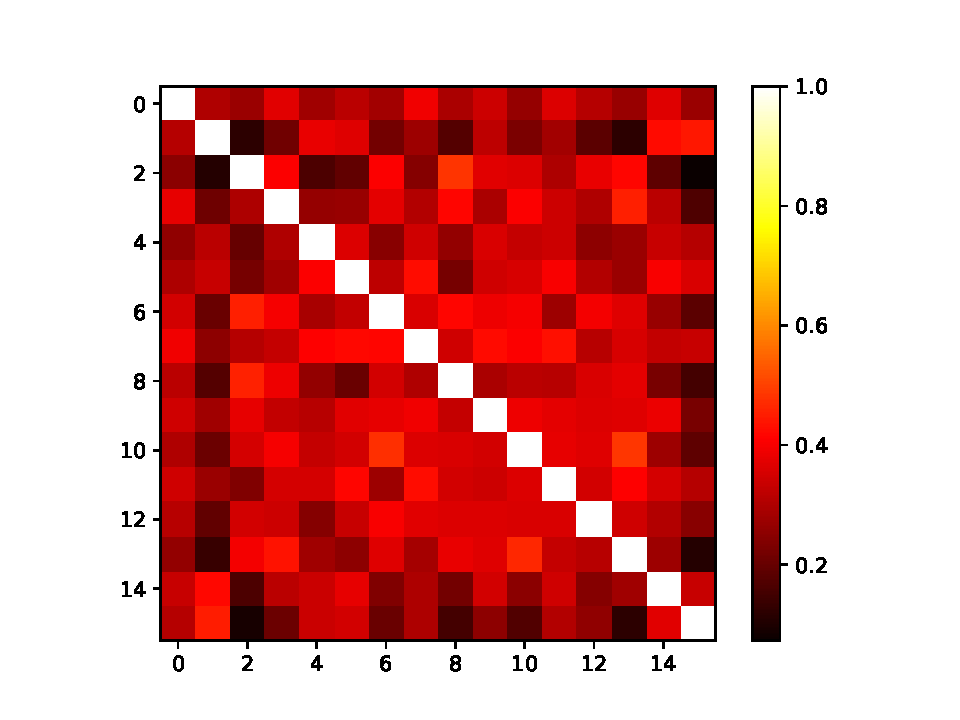
\includegraphics[width=0.8\textwidth]{similarityMat20.pdf}
	  \caption{指纹匹配度矩阵}
	  \label{fig:similarityMat}
  \end{figure}
  $similarityMat$矩阵的热力图表示见图\ref{fig:similarityMat}。


\subsubsection{灵敏度分析}
在使用匈牙利算法求解二部图最大匹配时,我们人物给定了每个指纹选取的特征点的个数$numFeatures$。本节我们分析$numFeatures$的取值是否对指纹的匹配度又重大影响。我们比较$numFeatures=10,15,20$时,相似度矩阵的平均误差绝对和最大绝对误差。

\begin{figure}[!h]
    \centering
    \begin{minipage}[c]{0.45\textwidth}
        \centering
        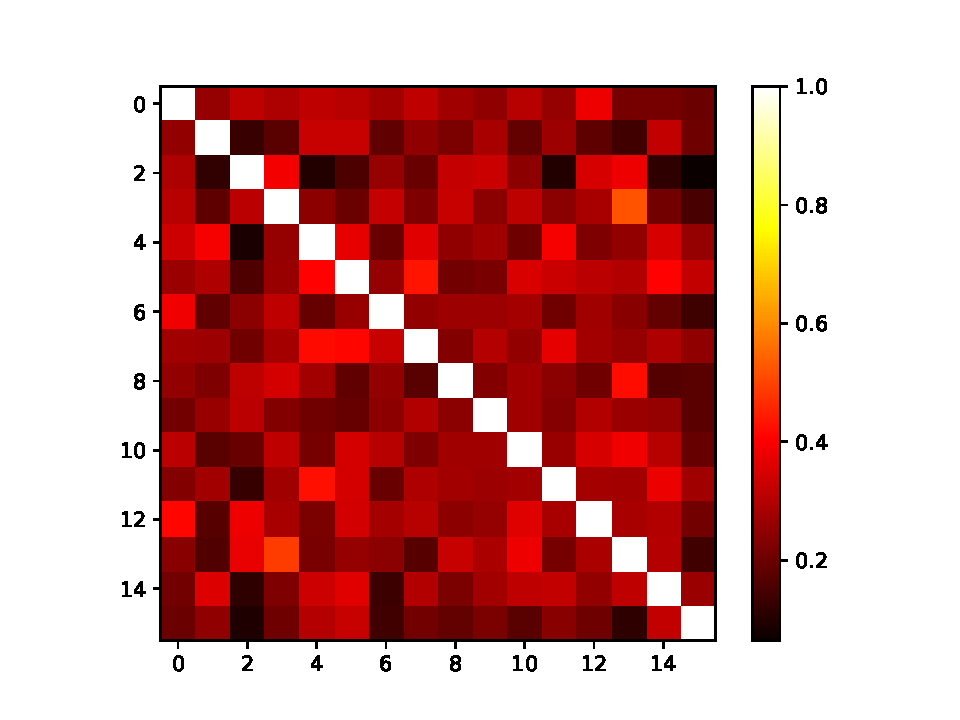
\includegraphics[width=0.99\textwidth]{similarityMat10.pdf}
        \subcaption{取10个特征点的相似度矩阵}
        \label{fig:similarityMat10}
    \end{minipage}
    \begin{minipage}[c]{0.45\textwidth}
        \centering
        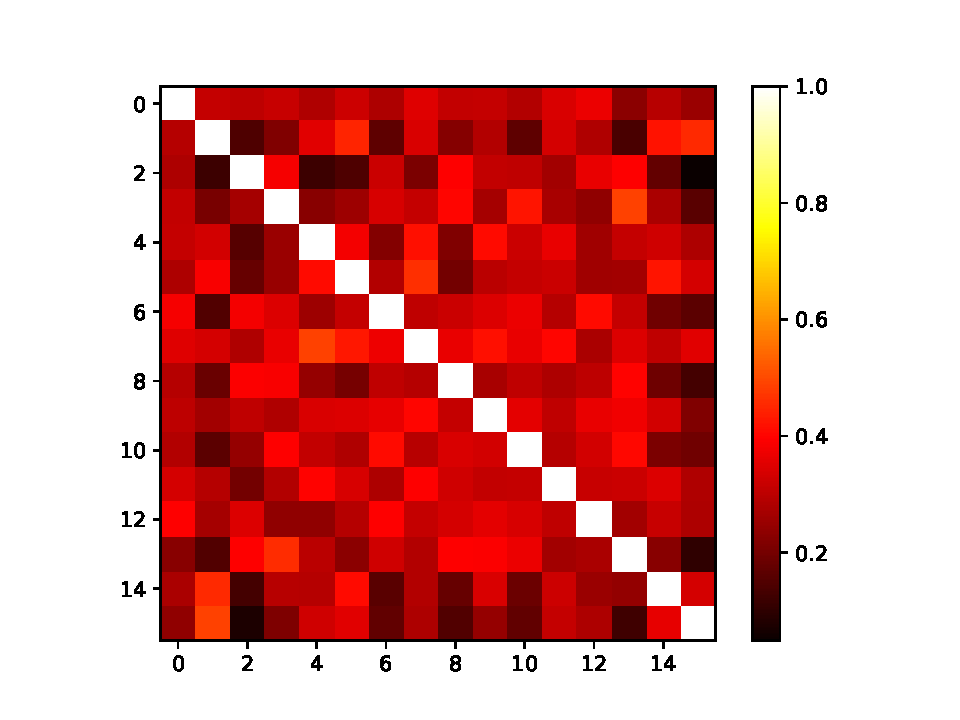
\includegraphics[width=0.99\textwidth]{similarityMat15.pdf}
        \subcaption{取15个特征点的相似度矩阵}
        \label{fig:similarityMat15}
    \end{minipage}
	\caption{$numFeatures=10,15$的对比}
  \end{figure}
% Table generated by Excel2LaTeX from sheet 'Sheet1'
\begin{table}[h!]
	\centering
	\caption{平均误差}
	  \begin{tabular}{crrr}
	  \toprule
			& \multicolumn{1}{c}{\textbf{0}} & \multicolumn{1}{c}{\textbf{1}} & \multicolumn{1}{c}{\textbf{2}} \\
	  \midrule
	  \textbf{0} & 0     & 0.046907 & 0.06007 \\
	  \textbf{1} & 0.046907 & 0     & 0.031546 \\
	  \textbf{2} & 0.06007 & 0.031546 & 0 \\
	  \bottomrule
	  \end{tabular}%
	\label{tab:avgErr}%
  \end{table}%

  % Table generated by Excel2LaTeX from sheet 'Sheet1'
\begin{table}[h!]
  \centering
  \caption{最大误差}
    \begin{tabular}{crrr}
    \toprule
          & \multicolumn{1}{c}{\textbf{0}} & \multicolumn{1}{c}{\textbf{1}} & \multicolumn{1}{c}{\textbf{2}} \\
    \midrule
    \textbf{0} & 0     & 0.249391 & 0.238563 \\
    \textbf{1} & 0.249391 & 0     & 0.108495 \\
    \textbf{2} & 0.238563 & 0.108495 & 0 \\
    \bottomrule
    \end{tabular}%
  \label{tab:maxErr}%
\end{table}%
可以看出改变特征点的个数$numFeatures$对指纹匹配度的影响不大,平均误差约为$6\%$,而最大误差也不超过$25\%$。



\section{问题三模型的建立与求解}
\subsection{问题分析}
该问题要我们对16幅指纹图像进行分类,通过参考指纹学对指纹的分类的判断依据和本题设计的编码方式,我们可以从指纹学上建立一个基于指纹学奇异点特征和指纹梯度方向与骨架抽象的方式,对指纹的总体特征和方向进行有效的分类,同时利用第二问中编码的结果对该模型进行修正以及同一类别不同指纹之间的对比相似度结果进行修正,并给出最终结果。
\subsection{奇异点特征与指纹方向场梯度分类模型}
\subsubsection{方向场梯度表示}
方向场代表了指纹图像的本质特征,经过预处理的指纹图像已得到精确的方向场,本文算法基于梯度求方向场。具体步骤如下:

(1)计算指纹图像每一点在X,Y方向的梯度$\partial$$x(i,j)$和$\partial$$y(i,j)$,梯度计算使用$Sobel$梯度算子。接着,使用下列公式计算每一点的方向,其中$W$常取常数8.


\begin{equation}
V_{x}(i, j)=\sum_{u=i-w}^{i+w}\sum_{v=j-w}^{j+w}\left(2 \partial_{x}(u, v) \partial_{y}(u, v)\right) 
\end{equation}

\begin{equation}
V_{y}(i, j)=\sum_{u=i-w}^{i+w} \sum_{v=j-w}^{j+w}\left(\partial_{x}^{2}(u, v)-\partial_{y}^{2}(u, v)\right) 
\end{equation}

\begin{equation}
\theta(x, y)=\frac{1}{2} \arctan \left(\frac{V_{y}(i, j)}{V_{x}(i, j)}\right)
\end{equation}


(2) 由步骤(1)得到的$q$$(x,y)$是局部脊线方向的最小平方估计,需要通过一个低滤波器进行修正,具体的修成方案如下:首先将方向场转化到一个连续的向量场中,再对其滤波,滤波后的向量场可以用下式表示:
\begin{equation}
\phi_{x}(i, j)=\cos (2 \theta(i, j)) 
\end{equation}
\begin{equation}
\phi_{y}(i, j)=\sin (2 \theta(i, j)) 
\end{equation}
\begin{equation}
\phi_{x}^{\prime}(x, y)=\sum_{u=-w_{\phi} / 2}^{w_{\phi} / 2} \sum_{v=-w_{\phi} / 2}^{w_{\phi} / 2}((h(u, v) \phi_{x}(i-u w, j-vw))
\end{equation}
\begin{equation}
\phi_{y}^{\prime}(x, y)=\sum_{u=-w_{\phi} / 2}^{w_{\phi} / 2} \sum_{v=-w_{\phi} / 2}^{w_{\phi} / 2}((h(u, v) \phi_{y}(i-u w, j-vw))
\end{equation}
\begin{equation}
O(i, j)=\frac{1}{2} \operatorname{atan} 2(\frac{\phi_{y}^{\prime}(i,j)}{\phi_{x}^{\prime}(i,j)} 
\end{equation}
\begin{equation}
O^{\prime}(i, j)=O(i, j)+\frac{\pi}{2}
\end{equation}

式中$\phi_{x}^{\prime}(x, y)$,$\phi_{y}^{\prime}(x, y)$是向量场的X,Y分量,中间两式子中$h$$(u,v)$是一个二维低通滤波器,积分为1,滤波器的大小为$W_{\phi}\times W_{\phi}$.将滤波前后的方向场图像进行对比 如图\ref{fig:Gaussian}所示:

\begin{figure}[!h]
    \centering
    \begin{minipage}[c]{0.45\textwidth}
        \centering
        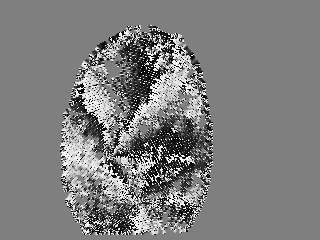
\includegraphics[width=0.99\textwidth]{2imgO_before_Gaussian}
        \subcaption{滤波前的方向场图像}
        \label{fig:2imgO_before_Gaussian}
    \end{minipage}
    \begin{minipage}[c]{0.45\textwidth}
        \centering
        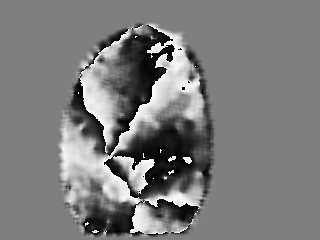
\includegraphics[width=0.99\textwidth]{3imgO_after_Gaussian}
        \subcaption{滤波后的方向场图像}
        \label{fig:3imgO_after_Gaussian}
    \end{minipage}
	\caption{$numFeatures=10,15$的对比}
	\label{fig:Gaussian}
  \end{figure}

\subsubsection{指纹奇异点特征提取}
奇异点提取是指纹图像处理中的一个重要部分,它可以作为指纹分类和识别过程中的定位基准点,根据其分布特性可以对指纹图像做粗分类,%故提取的准确性直接影响到指纹分类和细节匹配的准确率。
指纹的奇异点包括有指纹的中心点和三角点,根据指纹学的基础知识,中心点一般分为两种情况,有两个中心点或者一个中心点,而三角点并不是对于每个指纹都有的,不过也可以作为一个分类的依据和重要特征,在本文中,根据指纹方向场梯度得出的结果并提炼出其骨架可以从而将整个图像的指纹场的方向通过灰度梯度图来体现,根据方向梯度图,将方向场归域化$\Omega_{(0,4/\pi)},\Omega_{(\pi/4,\pi/2)},\Omega_{(\pi/3,3\pi/4)},\Omega_{(3\pi/4,\pi)}$,在方向图的交界处会出现很多的曲线交叉,这意味着这些特殊点周围区域方向变化十分强烈,这与奇异点周围方向变化强烈这一理论相符合,同时我们以3×3的8领域阵列,在特殊点交叉区域进行检验和去伪,从而得出了我们的奇异点。
\begin{equation}
|Poincare(i,j)+\pi|<0.01×\pi
\end{equation}
在满足该条件下的且是方向场剧烈变化的交叉点则可确定为奇异点,包括中心点和三角点都可以识别。

根据指纹学相关知识和方向场的理论我们可以对图片的类型和方向进行分类,首先基于中心点我们分为
两个中心点和一个中心点,同时在根据方向场的梯度和方向进行位置关系的判断,从而可以分辨出该指纹的类型,同时根据资料查找和题中所给的图片我们可以知道,一般带有三角点的图片可以认为是箕形,两个中心点的类型根据对应方向场的梯度方向大致可以判断出,螺旋型和斗型。

\begin{figure}[!h]
	\centering
	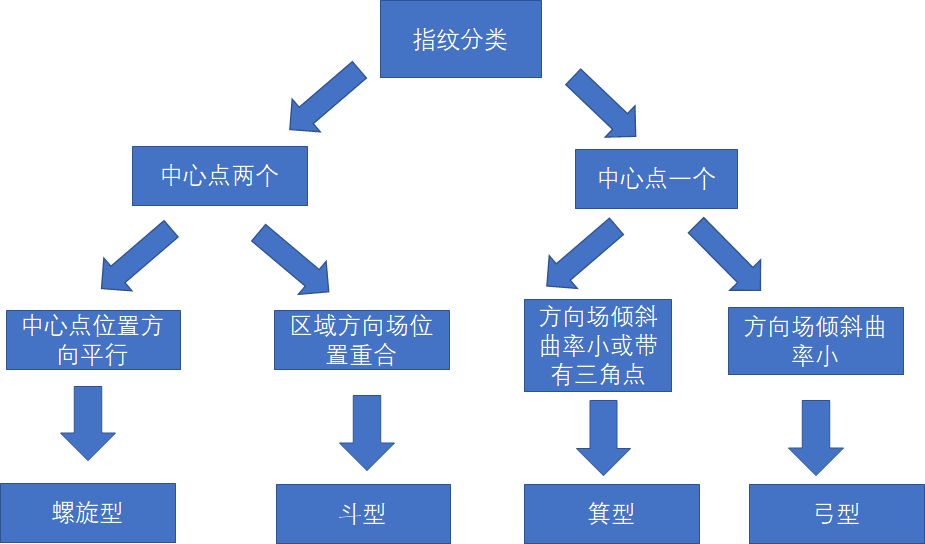
\includegraphics[width=0.8\textwidth]{classifyProcess.png}
	\caption{指纹分类流程}
\end{figure}

\subsection{模型求解}
\subsubsection{sobel算子与高斯滤波梯度提取}
在求解梯度的过程当中,为了减少计算量,我们将图片的规模缩小为原来的二分之一,然后利用python和opencv求解出sobel算子对图像在$x$和$y$方向上的梯度,然后我们利用低通滤波和高斯滤波的过滤对于图片中的方法进行了优化和提升。
\begin{equation}       %开始数学环境
Sobel_x= \begin{bmatrix}
-1 & 0 & 1\\
-2 & 0 & 2\\
-1 & 0 & 1\\
\end{bmatrix}   
Sobel_y= \begin{bmatrix}
1 & 2 & 1\\
0 & 1 & 0\\
-1 & -2 & -1\\
\end{bmatrix}           %右括号
\end{equation}
记原图像的像素矩阵为A,那么通过sobel算子可以很快求出图像在x和y方向上的梯度,$G_x$和$G_y$,然后通过合成计算出当前像素的梯度$G'$
\begin{equation}
G_x=Sobel_x*A \qquad
G_y=Sobel_y*A \qquad
G'=\sqrt{G_x^2+G_y^2}
\end{equation}
然后我们在上述方向场梯度模型的基础上加入高斯滤波的方式,从而最后得出结果。
最后我们能通过梯度的计算将该点斜率的倾斜角换算出来,然后对每一行和每一列进行倾斜角均值的计算,从而勾勒出该点的方向指纹方向。
\begin{figure}[!h]
	\centering
	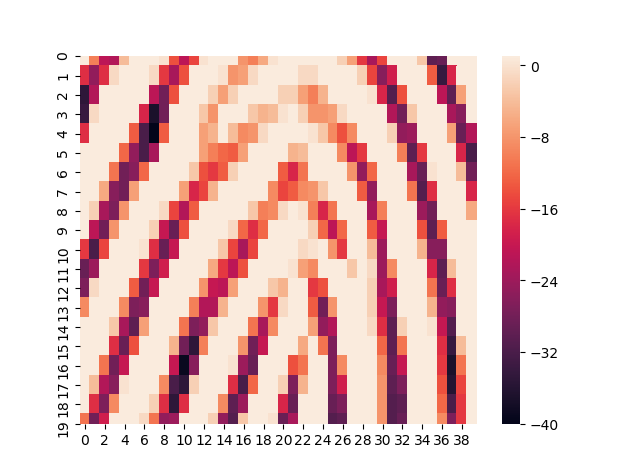
\includegraphics[width=0.8\textwidth]{centerhot.png}
	\caption{中心点附近图像梯度热力图}
\end{figure}
\begin{figure}[!h]
	\centering
	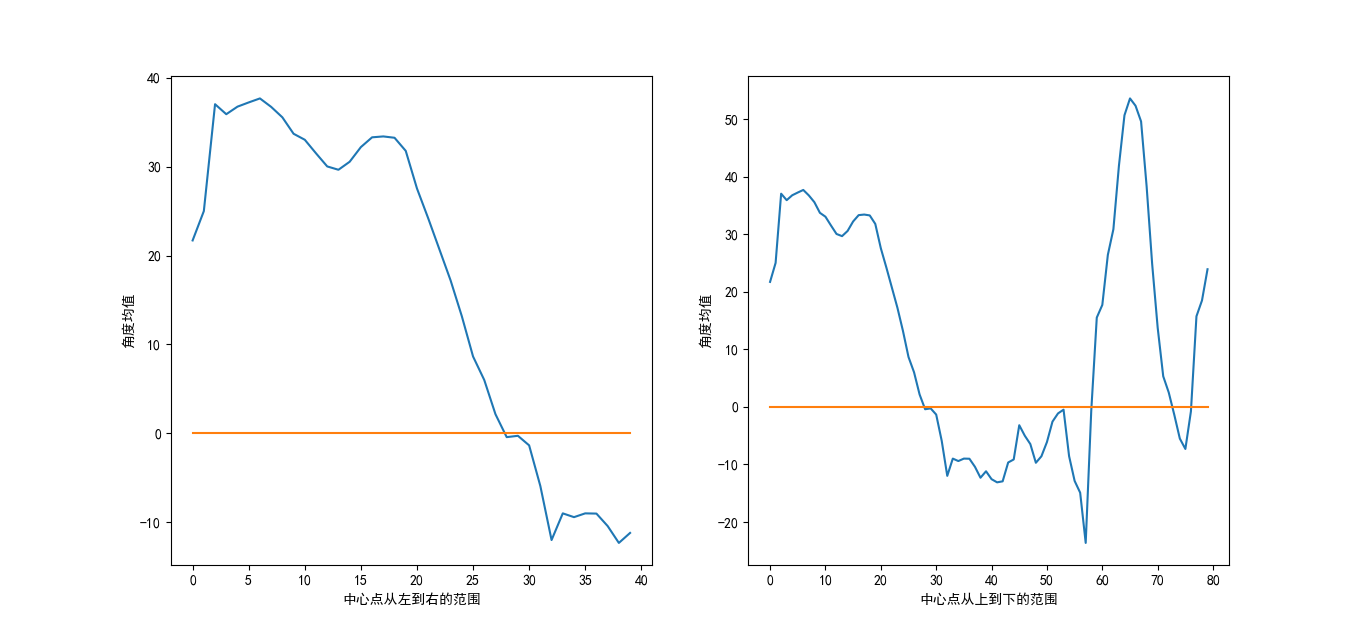
\includegraphics[width=0.95\textwidth]{two.png}
	\caption{中心点附近图像勾勒}
\end{figure}
\newpage
从图中我们就能看出来改中心点附件,从左往右他的角度确实呈现出整体向左的趋势,而从上往下也能体现出,当前位置下,呈现出先向上然后持平到最后下降的趋势,从而可以很好的反映中心点附件的朝向和趋势。
\newpage
\subsubsection{分水岭算法与poincare索引提取边界获取奇异点}
骨架提取与分水岭算法也属于形态学处理范畴,骨架提取,也叫二值图像细化。这种算法能将一个连通区域细化成一个像素的宽度,用于特征提取和目标拓扑表示,在我们第一步的操作中,我们滤波后的梯度图像作为输入图像,然后设置阈值$T=200$将其转化成二值图像,然后在对其骨架进行提取。
步骤:
1.读取滤波后的图像
2.设置阈值,提取梯度骤变的边界处
3.分水岭算法提取提取边界骨架
\begin{figure}[!h]
	\centering
	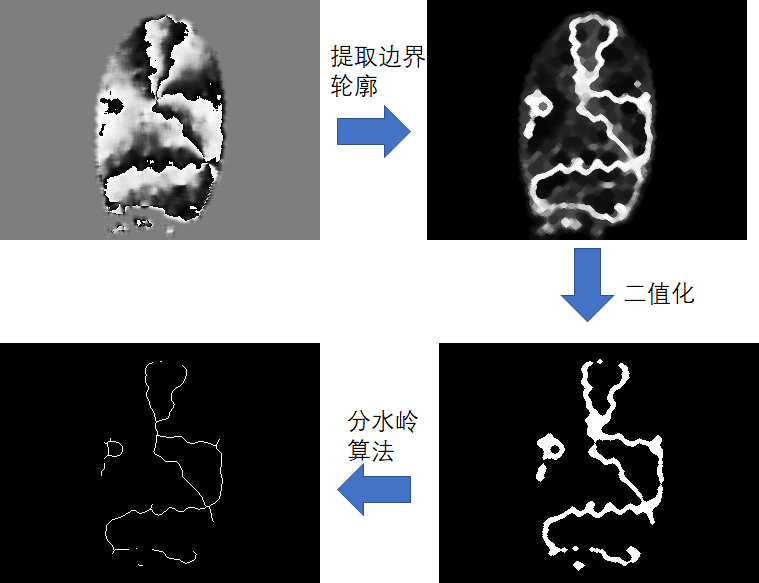
\includegraphics[width=0.95\textwidth]{fenshuilin.png}
	\caption{分水岭细化边界骨架}
\end{figure}

\subsection{结果分析}
\subsubsection{结果展示}
在获得骨架以后我们利用前期工作中提到的poincareinedx算法对梯度骤变的交界处的点进行奇异点的判断,然后并剔除了一些伪奇异点,从而准确得出了奇异点的所有坐标,为后面的分类提供支撑依据做准备。
\begin{figure}[!h]
	\centering
	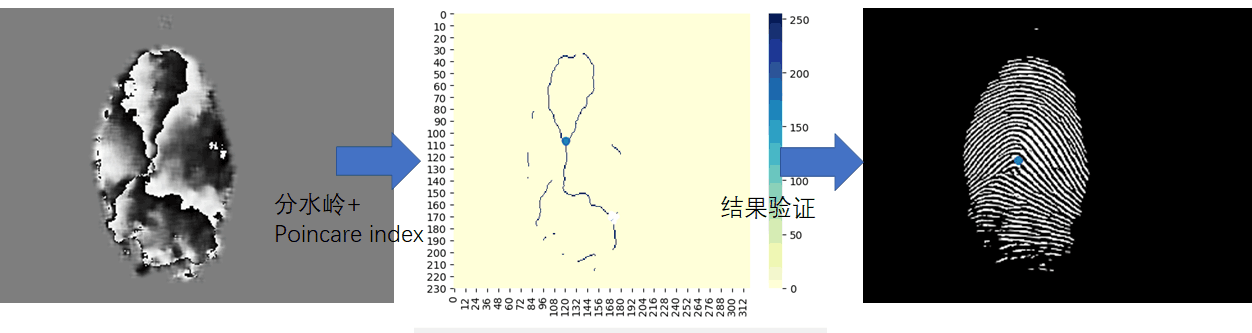
\includegraphics[width=0.95\textwidth]{fenshuijieguo.png}
	\caption{奇异点搜索效果}
\end{figure}
\begin{table}[!htbp]
	\caption{分类结果} \centering
	\begin{tabular}{cccccccc}
		\toprule[1.5pt]
$Name$ & $coreCount$ & $deltaCount$ & $center_x$ & $center_y$ & $delta_x$ & $delta_y$ &  $class$\\
		\midrule[1pt]

01.tif&	1&	0&	    266&	    384&	  &   	&	弓型\\
02.tif&	1&	1&	    308&	    192&   416&	 322&	箕型\\
03.tif&	1&	1&	    168&	    303&   316&	 386&	箕型\\
04.tif&	1&	0&	    250&	    248&	  &		&   弓型\\
05.tif&	1&	1&	    226&	    312&   262&  386&	箕型\\
06.tif&	1&	1&	    249&	    256&   306&	 340&	箕型\\
07.tif&	2&	0&	310,350&	164,254&	  &	    &	螺旋型\\
08.tif&	2&	1&	366,304&	300,268&	  &	    &	螺旋型\\
09.tif&	1&	0&	    219&	    232&	  &	    &   弓型\\
10.tif&	1&	1&	    282&        240&   362&	 384&	箕型\\
12.tif&	1&	0&	    304&	     77&	  &     &   箕型\\
13.tif&	1&	0&	    336& 	    278&	  &		&   箕型\\
14.tif&	2&	0&	    313,282&	    191,172&	  &		&   斗型\\
15.tif&	1&	0&  	305&	    328&	  &		&   弓型\\
16.tif&	1&	0&	    315&	    248&	  &	    &   箕型\\
		\bottomrule[1.5pt]
	\end{tabular}
\end{table}

\subsubsection{稳定性分析}
为了保证我们模型的准确性,我们对图片添加了噪声进行干扰,观察其是否会对我们模型的奇异点识别和梯度造成很大的影响从而影响分类的效果。我们对图片添加了高斯噪声,可以看出噪声前后中心点的差距只有$5\%$,而前后的趋势线也基本一致。
\begin{table}[!htbp]
	\caption{噪声前后结果对比} \centering
	\begin{tabular}{cccccccc}
		\toprule[1.5pt]
		$Name$ & $coreCount$ & $deltaCount$ & $center_x$ & $center_y$ & $delta_x$ & $delta_y$ &  $class$\\
		\midrule[1pt]
		
		01.tif&	1&	0&	    266&	    384&	  &   	&	弓型\\
		01.tif噪声后&	1&	0&	    262&	    395&	  &   	&	弓型\\
		\bottomrule[1.5pt]
	\end{tabular}
\end{table}
\begin{figure}[!h]
	\centering
	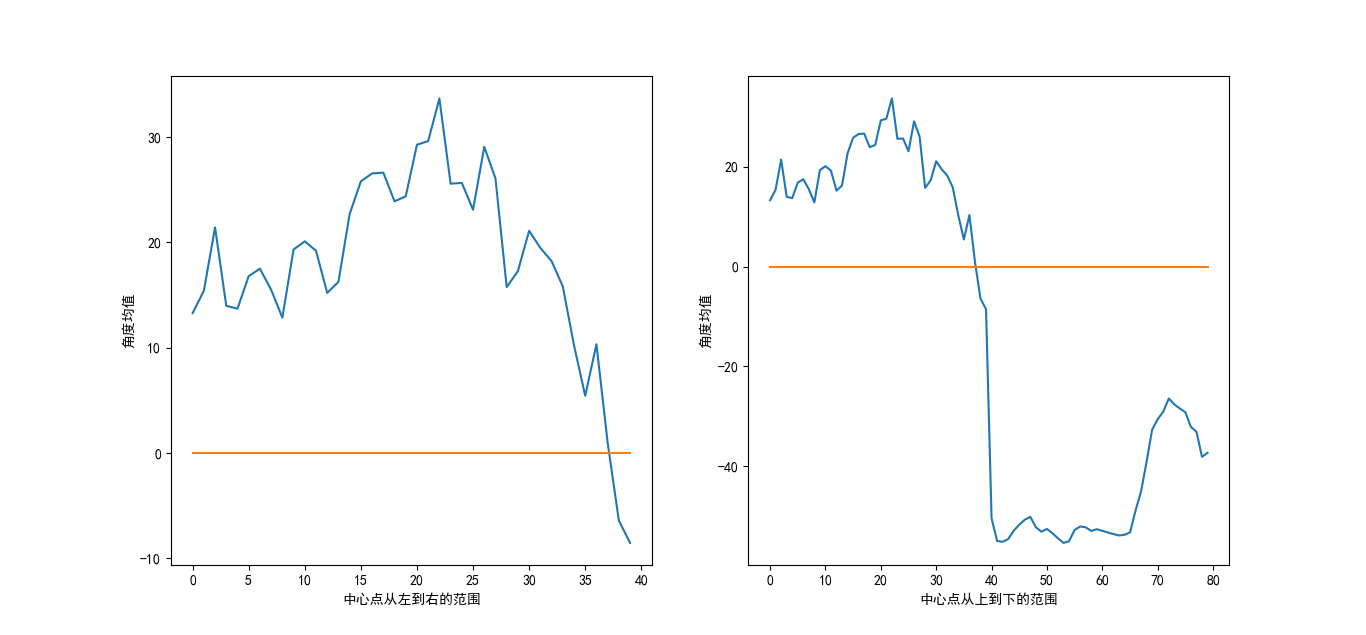
\includegraphics[width=0.8\textwidth]{zaoshengqian.png}
	\caption{噪声前中心点趋势图}
\end{figure}
\begin{figure}[!h]
	\centering
	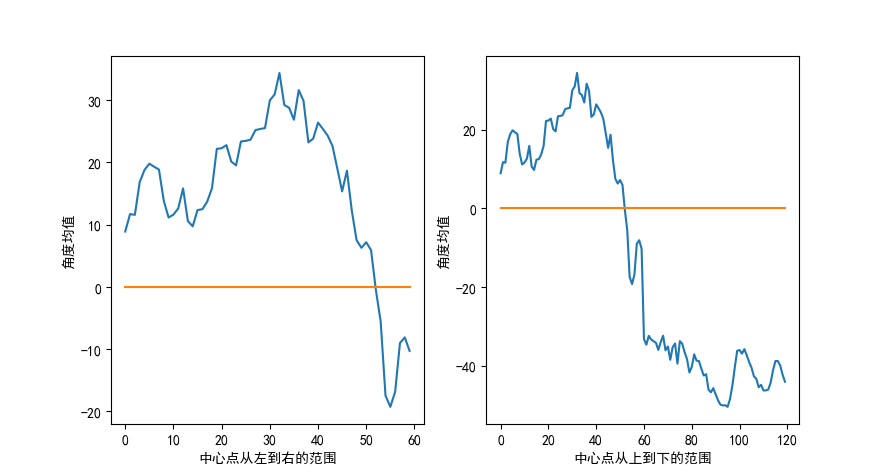
\includegraphics[width=0.8\textwidth]{zaoshenghou.png}
	\caption{噪声后中心点趋势图}
\end{figure}
\section{模型评价}
\subsection{模型的优点}
1.模型的建立考虑了指纹识别的整体流程,对因采集导致的清晰度下降和指纹因旋转而导致不一致的问题进行了深入讨论,同时我们以指纹细节点的相对位置作为编码的信息,使得模型不会受到图像平移的影响,模型使用范围具有普遍性。

2.模型二将题目转换成了一个二分图的图论模型,通过基于特征点的编码来进行分类操作,并利用匈牙利图论算法进行最大匹配,从而得出匹配的相似度匹配运算速度相比于其他智能算法的搜索要快。

3.第三问从图片纹理的方向梯度和指纹学的基本知识利用编码模型进行了合理的计算从而得出了该模型的准确分类。


\subsection{模型的缺点}
1.传统的Poincare index方法需要遍历全部像素点,使得模型算法变慢,降低了检测效率;且由于index值的不稳定性,容易产生伪中心点。

2.模型的二三问需要计算的梯度,和方向在操作层面上要计算的东西太多,需要继续整理成一个统一化的指标来进行预测会更好。

\subsection{改进与展望}
本文的模型是基于指纹学的相关知识和基本的编码思路来进行的操作,参考了许多关于指纹的模型来进行的模型建立,目前该模型对于指纹分类和指纹的相似度计算都给出了计算的方法和公式,要计算的指标和类型目前还有待进一步的提炼和统一,需要继续研究并给出统一的计算方法会更好。

1.更加高效的求解奇异点和特征点的方法

在目前的主流方法下还有很多可以借鉴的方法能够更加快速的来求解奇异点和特征点,如基于变维数优化模型的指纹奇异点提取,基于方向角度变化的指纹奇异点提取的快速算法,这些算法的核心大多是利用方向角的旋转变化和维度的搜索来准确定位奇异点和特征点,通过这些算法我们可以更快速的获取到指纹图中的重要特征点。

2.采用SVM等机器学习方法的指纹识别技术

如果在数据集达到一定规模程度之后,我们可以在当前特征点的基础上,利用支持向量机等机器学习的算法对指纹图像的全局特征和局部特征都能进行合适的分析和提取从而使得识别的效率更高,识别的准确度也相比少数量的指纹有更大的提升。


%参考文献
\bibliographystyle{plain}
\nocite{*}
\bibliography{thesis}
	

\newpage
%附录
\begin{appendices}
\section{16个指纹的编码}
\lstinputlisting[language=c]{code/hexCode.txt}

\section{python程序}

\subsection{main.py}
\lstinputlisting[language=python]{code/main.py}


\subsection{CommonFunctions.py}
\lstinputlisting[language=python]{code/CommonFunctions.py}

\subsection{extractMinutiaeFeatures.py}
\lstinputlisting[language=python]{code/extractMinutiaeFeatures.py}

\subsection{getGradient.py}
\lstinputlisting[language=python]{code/getGradient.py}

\subsection{getTerminationBifurcation.py}
\lstinputlisting[language=python]{code/getTerminationBifurcation.py}

\subsection{hungarian.py}
\lstinputlisting[language=python]{code/hungarian.py}

\subsection{matchMinutiae.py}
\lstinputlisting[language=python]{code/matchMinutiae.py}

\subsection{preprocess.py}
\lstinputlisting[language=python]{code/preprocess.py}

\subsection{removeSpuriousMinutiae.py}
\lstinputlisting[language=python]{code/removeSpuriousMinutiae.py}
\end{appendices}

\end{document} 